% Chapter 7

\chapter{Background Processes} % Chapter title

\label{ch:background_processes} 

%----------------------------------------------------------------------------------------

This analysis is fundamentally a search for \acf{SUSY} in events with two leptons whose invariant mass is consistent with a Z boson. Additional event selections are made to reduce \acf{SM} processes relative to potential \ac{SUSY} processes, defined by simplified models discussed in \autoref{sec:simplified_models}. \ac{SUSY} events typically have large amounts of \MET, \HT (the scalar sum of the \pT of all jets and the leading two leptons in an event), and many jets. All of these features can help isolate these events from backgrounds. To understand what cuts would optimize the sensitivity of the search, it is essential to first understand what these \ac{SM} backgrounds are. 

\begin{centering}
\begin{figure}[bth]
\myfloatalign
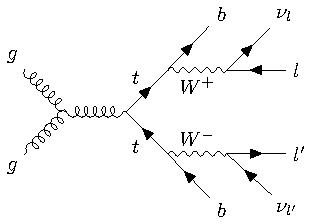
\includegraphics[width=.70\linewidth]{feynman/ttbar.pdf}
\caption{An example Feynman diagram of \ttbar production and decay.}
\label{fig:ttbar}
\end{figure}
\end{centering}

\paragraph{Top-antitop (\ttbar)} production is the largest background for this search. \autoref{fig:ttbar} shows an example of this process, which results in many jets, leptons, and neutrinos, which are seen in the detector as \MET. Thus, \ttbar events naturally have high \MET and \HT, jets, and leptons from two different W boson decays, which may coincidentally form an invariant mass consistent with a $Z$ boson. These events are very difficult to separate from potential signals, though keeping the mass window small and requiring \MET and \HT above the typical values for \ttbar events helps reduce this background.

\begin{centering}
\begin{figure}[bth]
\myfloatalign
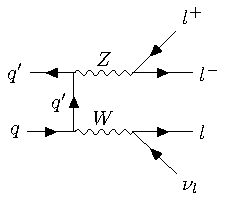
\includegraphics[width=.70\linewidth]{feynman/diboson.pdf}
\caption{An example Feynman diagram of the production and decay of a WZ event.}
\label{fig:diboson}
\end{figure}
\end{centering}

\paragraph{diboson ($VV$)} production is the next leading background. These events can contain real Z bosons and will peak on-Z like a signal. In addition, in events like \autoref{fig:diboson}, an additional W boson can decay to another lepton and a neutrino, providing \MET. The pictured process can occur with associated jets, but at reduced rates, so adding a jet requirement to the signal region helps reduce these events. If the W boson in this diagram instead decayed to two jets, there would be no true \MET from a neutrino, so a \MET cut in conjunction with a jet cut is very effective in reducing the total diboson background. A veto on a third lepton could also be used to reduce this background, but, depending on the signal model considered, this veto can also decrease signal acceptance, so it is not used in this analysis.

\begin{centering}
\begin{figure}[bth]
\myfloatalign
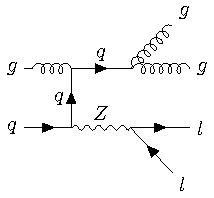
\includegraphics[width=.70\linewidth]{feynman/zjets.pdf}
\caption{An example Feynman diagram of the production and decay of a \dyjets event.}
\label{fig:zjets}
\end{figure}
\end{centering}

\paragraph{\dyjets} processes are very common but, as shown in \autoref{fig:zjets}, don't produce any true \MET. A high \HT cut helps reduce this background, but this process often occurs with associated jets, producing many events with large amounts of hadronic activity. \MET is the most powerful variable to reduce this background, because though events with mismeasured jets or leptons can fake \MET, mismeasurements drastic enough to produce hundreds of \gev~of \met are rare. 

Other processes can contribute to the Standard Model background at lower rates. Processes similar to \dyjets but with a W boson instead of a Z have real \MET from leptonic W decays, but only one lepton. However, a fake or non-prompt lepton can cause these events to look very similar to simulated signals. Additionally, there are rare processes such as \ttbar production in association with bosons that will also be difficult to separate from signal processes.

\section{Data and Monte Carlo Samples} 

This analysis uses data collected by the \ac{ATLAS} detector from $p-p$ collisions at a center-of-mass energy of 13 \tev in 2015 and 2016, corresponding to a total luminosity of 14.7 fb$^{-1}$. The data collected using a combination of unprescaled single and dilepton triggers, discussed in greater detail in \autoref{ch:eventsel}. In addition, photon events are collected for use in a control region using both prescaled and unprescaled triggers, with the lowest trigger threshold at 20 \gev. 

\ac{MC} samples are generated for each background process that appears in the signal and validation regions. \autoref{tab:MC} details the method used to produce each sample, and more information can be found in \autoref{sec:MC_gen}. These simulated background events, in conjunction with the simulated signal discussed in \autoref{sec:simplified_models}, are used to determine approximate sensitivities of the search and optimize signal regions and amount of data used. The background \ac{MC} also provides a valuable cross-check for many of the data-driven background estimates discussed in \autoref{ch:backgrounds}, and in some cases, provides the primary estimate of the background.

\begin{sidewaystable*}[ht]
\begin{center}
\caption{Simulated background event samples used in this analysis with the corresponding matrix element and parton shower generators,
cross-section order in $\alpha_{\text{s}}$ used to normalise the event yield, underlying-event tune and PDF set.
}
\scriptsize
\begin{tabular}{l c c c c c }
\hline
Physics process &  Generator  & Parton & Cross section & Tune & PDF set\\
                &             & Shower &              &      & \\
%\hline\hline
\noalign{\smallskip}\hline\noalign{\smallskip}
$t\bar{t}+W$ and $t\bar{t}+Z$~\cite{ATL-PHYS-PUB-2016-005,Garzelli:2012bn}& {\sc MG5\_aMC@NLO}        & {\sc Pythia} 8.186 & NLO \cite{Campbell:2012,Lazopoulos:2008} & {\sc A14} & NNPDF23LO\\
$t\bar{t}+WW$~\cite{ATL-PHYS-PUB-2016-005}      & {\sc MG5\_aMC@NLO}          & {\sc Pythia} 8.186 & LO \cite{Alwall:2014hca} & {\sc A14}  &  NNPDF23LO\\
$t\bar{t}$~\cite{ATL-PHYS-PUB-2016-004}         & {\sc Powheg Box v2} r3026   & {\sc Pythia} 6.428 & NNLO+NNLL \cite{ttbarxsec1,ttbarxsec2}          &\sc{Perugia2012}     &NLO CT10\\
Single-top ($Wt$)~\cite{ATL-PHYS-PUB-2016-004}  & {\sc Powheg Box v2} r2856   & {\sc Pythia} 6.428 & Approx. NNLO \cite{Kidonakis:2010b}& \sc{Perugia2012}    &NLO CT10 \\ 
$WW$, $WZ$ and $ZZ$~\cite{ATL-PHYS-PUB-2016-002} & \sherpa\ 2.1.1 & \sherpa\ 2.1.1 & NLO \cite{diboson1,diboson2} & \sherpa\ default & NLO CT10 \\
%$WZ$ and $ZZ$~\cite{ATL-PHYS-PUB-2016-002} &&& \\ 
$Z/\gamma^{*}(\rightarrow \ell \ell)$ + jets~\cite{ATL-PHYS-PUB-2016-003}& \sherpa\ 2.1.1           & \sherpa\ 2.1.1  &NNLO \cite{DYNNLO1,DYNNLO2}       & \sherpa\ default     &NLO CT10\\
\gjets & \sherpa\ 2.1.1 & \sherpa\ 2.1.1 & LO~\cite{sherpa} & \sherpa\ default & NLO CT10 \\
$V(=W,Z)\gamma$ & \sherpa\ 2.1.1 & \sherpa\ 2.1.1 & LO~\cite{sherpa} & \sherpa\ default & NLO CT10 \\
signal & {\sc MG5\_aMC@NLO} & {\sc Pythia} 8.186 & NLO & A14 & NNPDF23LO\\
\noalign{\smallskip}\hline\noalign{\smallskip}
\end{tabular}
\label{tab:MC}
\end{center}
\end{sidewaystable*}
